\section{Evaluation}
As mentioned, $\rho$ is calibrated to 0.2 based on optimizing the log loss function for previous year's results.  The log loss for 2014 for the entire range of $\rho$ can be seen in Figure~\ref{fig:result}.
\begin{figure}[h]
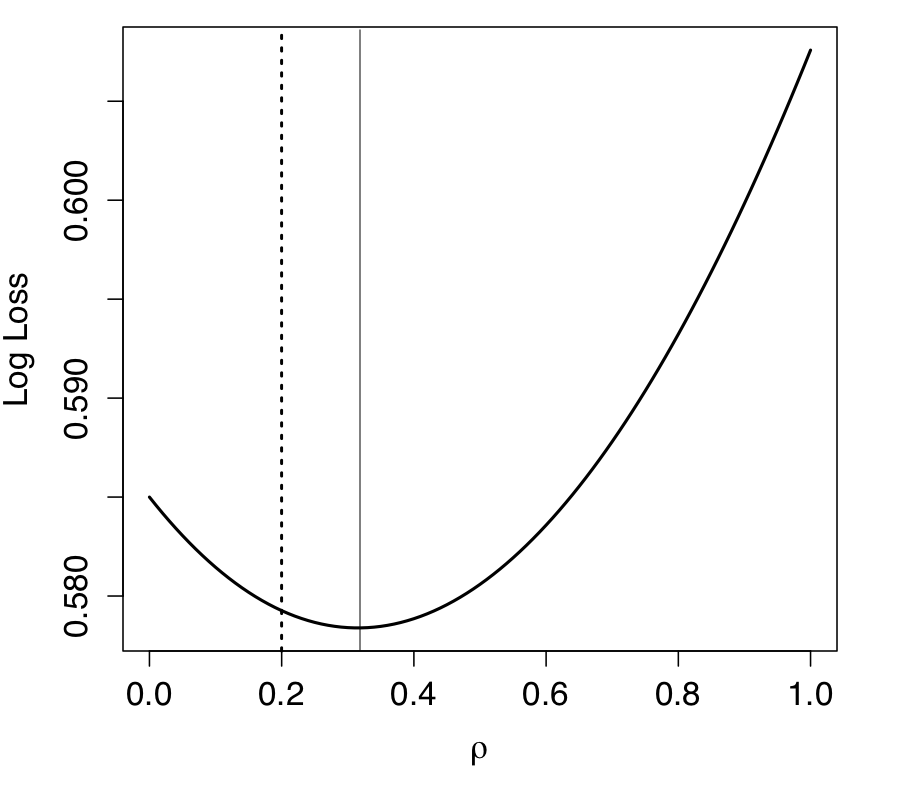
\includegraphics[width=1\textwidth]{results_2014.png}
\caption{Log loss for no matchup effect = red, log loss for optimized $\rho$ = blue}
\label{fig:result}
\end{figure}
A  gain is achieved by using the 0.2 value that minimized the log loss for the previous 7 NCAA tournaments.  A modest gain is also seen in classification error from (0.365 to 0.350) although this is only a single game difference.  The matchup effect, particularly with smaller $\rho$ values, will have minimal effects on classification error.  This is because it will only shift the expected point differential a small margin, so only dead heat games would expect to see prediction changes.

To understand the differences in the matchup effects, consider Table~\ref{tab:change} which contains the ten games that saw the largest shift in expected point differential.  able~\ref{tab:change} contains probabilities of team 1 winning as well as expected point differential and the realized loss for each model.
\begin{table}[ht]
\caption{Ten games with largest point differential change}
\footnotesize
\centering
\begin{tabular}{rlrrrrrrll}
  \hline
 team1 & Diff & Prob & Log.loss & Diff.ME & Prob.ME & Log.loss.ME & wteam.1 & lteam.1 \\ 
  \hline
 Cal Poly SLO & -18.69 & 0.04 & 0.04 & -17.10 & 0.06 & 0.06 & Wichita St & Cal Poly SLO \\ 
 Connecticut & 4.29 & 0.65 & 0.43 & 6.18 & 0.71 & 0.34 & Connecticut & St Joseph's PA \\ 
 Dayton & -2.16 & 0.42 & 0.86 & 0.94 & 0.53 & 0.63 & Dayton & Stanford \\ 
 Dayton & -6.34 & 0.28 & 1.27 & -4.05 & 0.36 & 1.03 & Dayton & Syracuse \\ 
 Kentucky & -3.71 & 0.37 & 1.00 & -2.08 & 0.42 & 0.86 & Kentucky & Michigan \\ 
 Massachusetts & -3.05 & 0.39 & 0.49 & -4.83 & 0.33 & 0.40 & Tennessee & Massachusetts \\ 
 Memphis & -6.34 & 0.28 & 0.33 & -8.91 & 0.21 & 0.23 & Virginia & Memphis \\ 
 Michigan & 5.37 & 0.69 & 0.37 & 3.49 & 0.62 & 0.47 & Michigan & Tennessee \\ 
 Michigan & 8.05 & 0.77 & 0.26 & 5.85 & 0.70 & 0.35 & Michigan & Texas \\ 
 Syracuse & 12.65 & 0.88 & 0.13 & 15.01 & 0.92 & 0.09 & Syracuse & W Michigan \\ 
   \hline
\end{tabular}
\label{tab:change}
\end{table}
On this particular subset of games, the matchup effects model performs considerably better than the typical model under the log loss (.446 to .520).  As the other games see minimal matchup effects, the results are essentially the same.  